\documentclass[a4paper,twoside,12pt,]{article}
\usepackage[a4paper,top=3cm,bottom=3cm,left=3.8cm,right=3.8cm]{geometry}
\usepackage[italian]{babel}
\usepackage{wrapfig}
\usepackage{indentfirst}
\usepackage[utf8]{inputenc}
\usepackage{graphicx}
\usepackage{booktabs}
\usepackage{multirow}
\usepackage[pdftitle={Italian OpenStreetMap Minitutorial},pdfauthor={Luca Delucchi, Maurizio Napolitano, Alessio Zanol},colorlinks=true,citecolor=blue,urlcolor=blue,filecolor=blue,linkcolor=blue]{hyperref}
\usepackage{xspace}
%comando per scrivere openstreetmap
\newcommand{\osm}{OpenStreetMap\xspace}
\newcommand{\gps}{GPS\xspace}

%opening
\title{\begin{Large}Minitutorial Italiano di \osm\end{Large}}
\author{Luca Delucchi, Maurizio Napolitano, Alessio Zanol}
\begin{document}

\maketitle
\begin{center}
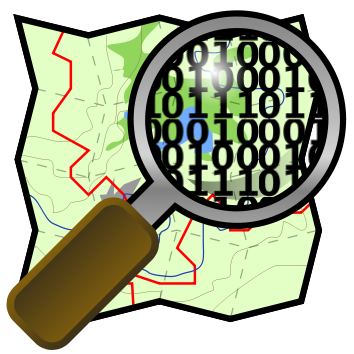
\includegraphics{Openstreetmap.png}
\end{center}
\begin{center}
	\begin{large}
	\textbf{Comunità Italiana di OpenStreetMap}
	\end{large}
\end{center}
\newpage
% \tableofcontents
% \newpage

\section{Cos'è \osm}
\osm è un progetto mondiale per la raccolta collaborativa di dati geografici da cui si possono derivare innumerevoli lavori e servizi. I risultati più evidenti sono le mappe online che però rappresentano solo la punta dell'iceberg di quel che si può ottenere da questi dati.

La \textbf{caratteristica fondamentale è che i dati di \osm possiedono una licenza libera}, attualmente la Creative Commons BY SA. E' cioè possibile utilizzarli liberamente per qualsiasi scopo con il solo vincolo di citare l'autore e usare la stessa licenza per eventuali lavori derivati dai dati \osm. 

L'altra caratteristica molto importante è che tutti possono contribuire arricchendo o correggendo i dati, e come i progetti simili (Wikipedia e mondo del software libero ad esempio) \textbf{la comunità è l'elemento fondamentale} perchè oltre a essere quella che inserisci i dati e arrichisce il progetto controlla anche la sua qualità.
\section{Cosa non è \osm}
\textbf{\osm non è una raccolta di tracce \gps tra loro slegate}. Le tracce \gps sono solo utili per capire come tracciare il reticolo delle strade e di inserire i waypoint.

\textbf{\osm non è una copia di Google Maps} e non è quello il suo scopo, è molto di più \dots

\section{La struttura di OpenStreetMap}
\subsection{Elementi}
\textbf{\osm è un database}, gli elementi che possono essere inseriti (strade, negozi ecc ecc), tramite alcuni software che vedremo in seguito, sono di quattro tipologie:
\begin{itemize}
 \item \texttt{punti} (node): singoli punti
 \item \texttt{linee} (way): un insieme di punti non chiuso
 \item \texttt{aree} (polygon): un insieme di punti chiuso, solitamente con il tag area=yes
 \item \texttt{relazioni} (relation): un insieme degli elementi precedenti, per esempio una linea degli autobus che è composta da più strade e dalle sue fermate
\end{itemize}
\begin{center}

\includegraphics{elements.png}
\end{center}
\subsection{Tag}
Le \textbf{etichette (tag)} servono per descrivere le caratteristiche dei vari elementi. I \textbf{tag sono sempre composti da una coppia di nomi}. Il primo è detto \textbf{key}, il secondo \textbf{value}. Solitamente il key descrive una famiglia di caratteristiche, mentre il value va più nello specifico. Ad esempio la key highway indica la famiglia delle strade di qualsiasi tipo, dalle autostrade ai sentieri, di seguito ne presentiamo alcuni:
\begin{center}
 \begin{tabular}{ccc}
  \toprule
   \textbf{key} & \textbf{values} & \textbf{descrizione} \\
  \midrule
   \multirow{10}*{highway} & motorway & autostrada \\
    			& trunk & superstrade \\
    			& primary & strade di importanza nazionale \\
    			& secondary & strade di importanza regionale \\
    			& tertiary & strada di importanza locale \\
    			& unclassified & strade del reticolo di base \\
			& residential & strade per abitazioni \\
			& service & strade di servizio \\
    			& track & strade agricole o forestali \\
			& pedestrian & vie pedonali cittadine \\
    			& footway & sentieri \\
    			& cycleway & piste ciclabili \\
			& steps & scale \\
			& bus\_stop & fermate dell'autobus \\
			& stop & segnale stop \\
			& traffic\_signal & semaforo \\
			& emergency\_access\_point & SOS \\
  \bottomrule
 \end{tabular}
\end{center}
I tag non rappresentano solo un elemento ma possono essere usati per più elementi per esempio highway è prevalentemente associato alle linee ma come potete vedere sopra vi sono alcune casi in cui è utilizzato con i nodi highway=bus\_stop o highway=traffic\_signal

I tag usati sono tantissimi e continuano ad aumentare e migliorare, permettono di mappare qualsiasi elemento possa essere rappresentato da una coppia di coordinate geografiche, una vasta lista è disponibile al link  \url{http://wiki.openstreetmap.org/wiki/Map_Features} inoltre è possibile controllare, discutere e votare i nuovi tag proposti qui in questa pagina \url{http://wiki.openstreetmap.org/wiki/Proposed_features}.

Oltre ai tag per le strade esistono molti tag per elementi puntuali, lineari e areali eccone alcuni:
\begin{center}
 \begin{tabular}{cccc}
  \toprule
   elemento & key & value & descrizione \\
  \midrule
  \multirow{11}*{puntuale} & \multirow{2}*{amenity} & pub & pub \\
			& & bank & banca \\
 & & & \\
			& \multirow{2}*{shop} & supermarket & supermercato \\
			& & bakery & panificio \\
 & & & \\
			& \multirow{2}*{tourism} & hotel & albergo o hotel \\
			& & information & punto informazioni turistiche \\
 & & & \\
			& \multirow{2}*{railway} & station & stazione ferroviaria \\
			& & level\_crossing & passaggio a livello \\
  \midrule
  \multirow{8}*{lineare} & \multirow{2}*{aerialway} & cable\_car & funivia \\
			& & chair\_lift & cabinovia \\
 & & & \\
			& \multirow{2}*{waterway} & river & fiume \\
			& & canal & canale \\
 & & & \\
			& \multirow{2}*{railway} & rail & ferrovia \\
			& & tram & linea tram \\
  \midrule
  \multirow{8}*{areale} & \multirow{2}*{natural} & water & fiumi molto larghi o laghi \\
			& & wood & foresta \\
 & & & \\
			& \multirow{2}*{leisure} & playground & parco giochi \\
			& & sport\_center & stadio \\
 & & & \\
			& \multirow{2}*{landuse} & residential & zone residenziali \\
			& & vineyard & vigneti \\
  \bottomrule
\end{tabular}

\end{center}

Inoltre ricorda che per ciascun elemento è possibile assegnare più di un tag in modo da descriverlo in modo completo, ad esempio:
\begin{center}
 \begin{tabular}{cc}
  \toprule
   \textbf{key} & \textbf{value} \\
  \midrule
   highway & unclassified \\
   name & Via Roma \\
   access & no \\
   foot & yes \\
   bicycle & no \\
   oneway & yes \\
  \bottomrule
 \end{tabular}
\end{center}
\subsection{Relation}
Per quanto riguarda le relation attualmente sono solo quattro quelle ufficiali anche se molte altre sono state proposte e già utilizzate, tipo quelle per i numeri civici, di seguito vedremo le ufficiali e poi approfondiremo le route che sono le più utilizzate e forse importanti
\begin{center}
 \begin{tabular}{c p{9cm}}
  \toprule
   \textbf{tipo} & \textbf{descrizione} \\
  \midrule
   multipolygon & serve per creare un poligono all'interno di un altro poligono, per esempio un'isola in un lago \\
   restriction	& serve per vietare le svolte \\
   boundary	& serve per raggruppare aree e creare enclavi ed exclavi \\
   route & serve per creare dei percorsi, possono essere pedonali (per esempio sentieri montani), ciclabili, linee di trasporti pubblici ecc ecc \\
   enforcement & per inserire elementi per misurare e documentare sulle violazioni veicolari \\
  \bottomrule
\end{tabular}
\end{center}

Di seguito vedremo come utilizzare la relation route
\begin{center}
 \begin{tabular}{cp{9cm}}
  \toprule
   \textbf{key} & \textbf{value} \\
  \midrule
   type & \textit{route} \\
   route & \textit{road - bicycle - foot - hiking - bus - ferry - canal -pilgrimage - detour - railway - tram - trolleybus - mtb (mountainbike) - roller\_skate - running - horse - parade - protest\_march (recurring)} \\
   ref & \textit{codice identificatico se presente}\\
   operator & \textit{nome dell'operatore se presente} \\
   name & \textit{nome se presente} \\
   symbol & \textit{simbolo se presente} \\
  \bottomrule
\end{tabular}

\end{center}

\section{Come posso contribuire}
\subsection{Non ho il \gps}
\begin{wrapfloat}{figure}{R}{0pt}
 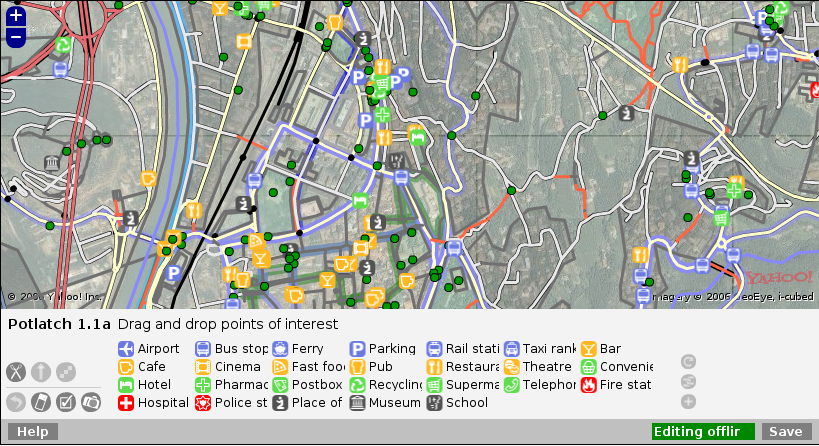
\includegraphics[width=0.7\columnwidth]{potlatch.png}
 \caption{\textit{L'interfaccia di Potlatch}}
\end{wrapfloat}
Puoi collaborare alla mappatura anche se non hai il \gps, l'\textbf{importante è avere una connessione ad internet}\dots come? per esempio inserendo i nomi delle vie dove non sono presenti, inserendo i punti di interesse (negozi, punti turistici, fontane, servizi\dots), correggendo eventuali errori. Inoltre per molte zone si hanno le fotoaeree di Yahoo in alta risoluzione, la cui licenza permette di "ricalcarle".

Dopo esserti iscritto attraverso l'homepage, per iniziare a farti un'idea potresti zoommare in un luogo mappato che conosci e cliccare su \textit{"Edit"} e guardare come sono strutturate le strade e i punti di interesse cliccandoci su ma, almeno all'inizio, se non sei sicuro di quello che fai non modificare la mappa.
Quello che hai appena usato è \texttt{Potlatch}, l'editor online.

Esistono altri editor che funzionano come programmi a se stanti. Il più usato e completo è senz'altro \texttt{JOSM}, \url{http://josm.openstreetmap.de/} un altro si chiama \texttt{Merkaartor} \url{http://www.merkaartor.org/}.
Un'altra cosa molto importante quando si inizia a tracciare le strade, in particolare con l'editor online, è verificare che le varie strade siano tra loro interconnesse da un nodo comune. Nell'editor online è possibile assicurarsi di ciò quando, sovrapponendo la linea che si sta tracciando alla strada a cui si vuole congiungere, i nodi di questa si evidenziano di blu.

Molto altro ci sarebbe da dire, inizia pure a lavorare con cautela e \textbf{per qualsiasi dubbio domanda in mailing list o sul canale irc, prima di chiedere controlla che qualcuno non abbia già avuto il tuo stesso problema consultando gli archivi della mailing list.}

Se non hai \gps puoi anche usare Walking Papers che permette di stampare una zona e poi segnare su questa le modifiche da fare, ovviamente dove ci sono già un po' di dati come base.

\textbf{IMPORTANTE: non copiare mai da altre mappe se non sei sicuro di poterlo fare. Né Google né le carte topografiche hanno una licenza che ne permette la copia.}

\textbf{Preferisci sempre il sopralluogo di persona sul posto. Nel dubbio non mappare.}
\subsection{Ho il \gps}
Come spiegato nei primi paragrafi, le tracce \gps non entrano direttamente nel database di \osm. Sono estremamente utili però come base su cui poi ricalcare le way e i nodi mediante i software a disposizione come \texttt{Potlatch} o \texttt{JOSM}.
\begin{wrapfloat}{figure}{L}{0pt}
 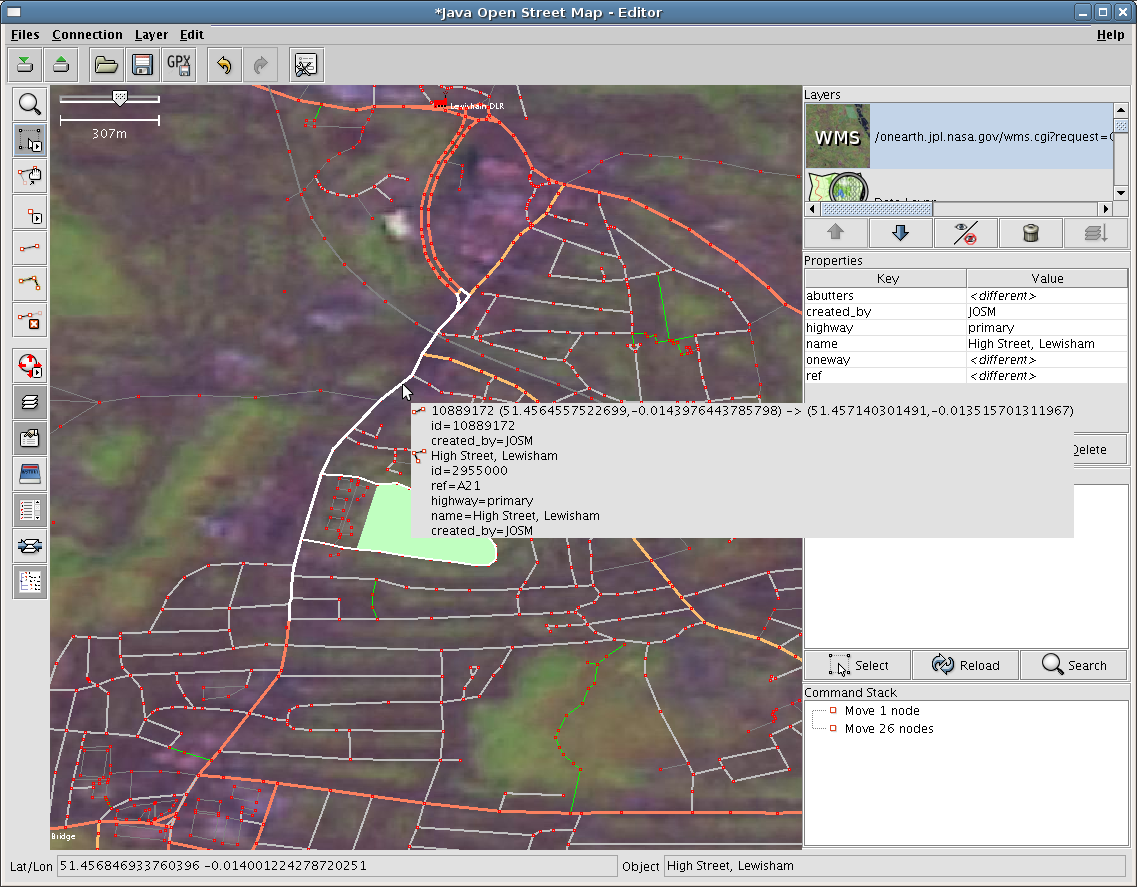
\includegraphics[width=0.6\columnwidth]{Josm-screenshot.png}
 \caption{\textit{L'interfaccia di JOSM}}
\end{wrapfloat}
Supponiamo di aver a disposizione un \gps per fare una bellissima gita in montagna. Accendiamo il nostro apparecchio, attendiamo l'aggancio dei satelliti ed iniziamo la registrazione della traccia. Per il progetto è molto importante avere i punti delle tracce abbastanza ravvicinati perciò \textbf{è bene settare nelle impostazioni del vostro \gps di salvare i punti delle tracce con una frequenza maggiore a quella di default}, le impostazioni più utilizzate sono quelle basate sul \textit{tempo} (questo metodo va settato in base al mezzo di locomozione: in macchina e in bici vanno bene valori inferiori a 5 secondi, a piedi si può arrivare fino a 10) oppure sulla \textit{distanza} (in questo caso è bene non superare i 10 m, sui garmin è il minimo disponibile), per i novizi consiglio di utilizzare la distanza poichè questo metodo crea una traccia ``più pulita'' rispetto al metodo del tempo.

Supponiamo che il nostro percorso inizi su una strada forestale. E' bene in questo caso appuntare questa informazione poiché nella fase di editing sarà ricalcata ed etichettata con highway=track. Un modo semplice per tener nota di queste cose è utilizzare i waypoint registrabili col \gps, cioè memorizzare nel nostro caso il punto di inizio della strada foresta con un waypoint e se il modello lo permette assegnargli un nome significativo (es. inizio forestale). Se il \gps non lo permette appuntare su un pezzo di carta il codice del waypoint in questione e la sua descrizione. Allo stesso modo registreremo la fine della strada forestale con un altro waypoint così come l'inizio del sentiero.

Sempre mediante i waypoint è utile appuntare informazioni interessanti come il codice del sentiero o il suo nome.

E' da precisare che il nome che si assegna ai waypoint non è fondamentale, ma serve come promemoria personale, infatti nemmeno i waypoint entrano a far parte del database di OSM, ma serviranno esclusivamente da appunti in fase di editing. Adottate quindi lo stile che più trovate utile, completo e comodo per appuntare quel che trovate.

Non solo le strade sono ovviamente importanti per \osm ma ad esempio nel nostro giro in montagna potrebbero essere interessanti segnavie (amenity=signpost), bivacchi (amenity=shelter), fontanelle di acqua potabile (amenity=drinking\_water),  rifugi (tourism=alpine\_hut) e molto altro ancora\dots

A questo punto, giunti a casa dalla nostra gita, scarichiamo sul PC le tracce e i waypoints rilevati, apriamo il nostro editor preferito e dal menù carichiamo sia le tracce che i waypoints che quindi ci appariranno sullo schermo. Ora si possono scaricare i dati di \osm già presenti sul server mediante l'apposito pulsante.

Attraverso i tool di disegno si vanno così a ricalcare le nostre tracce assegnando i tag di descrizione; le modifiche effettuate possono ora essere caricate sul server di \osm mediante l'apposito pulsante.

Sulla mappa in homepage (detta slippy map) le modifiche non appariranno istantaneamente ma si dovrà attendere un po' di tempo prima che vengano renderizzate; questo processo può durare da qualche ora ad una settimana.

E' da sottolineare anche che se le tracce non entrano direttamente nel database principale di \osm, è possibile caricarle sul sito tramite la pagina \url{http://www.openstreetmap.org/traces}, al fine di renderle pubbliche e disponibili a chiunque le voglia ricalcarle o controllarle, inoltre passando più volte nella stessa ``strada'' avremo delle tracce sempre un po' diverse, avendone tante si può avere una precisione maggiore facendo passare la nostra way nella linea mediana di tutte le tracce.
\section{Donazione tracce}
Se hai delle tracce create da te col \gps e non hai voglia o tempo di imparare ad importarle, puoi aiutare \osm già da subito "donandole".

Qualcuno della comunità, possibilmente che conoscerà la tua zona, le caricherà all'interno del database di \osm.

Le tracce migliori sono quelle su un unico tipo di percorso es: tutto sentiero o tutto strada forestale , ma anche le altre in generale vanno bene, in questo caso sarebbe meglio avere un minimo di conoscenza della zona oppure una breve descrizione del tracciato.
\section{Passaparola}
Se a te il progetto non interessa \textbf{passaparola a tutti coloro che potrebbero essere incuriositi o che potrebbero dare una mano}.

Quando c'è la possibilità usa le mappe online di \osm se hai da mostrare delle zone a degli amici, ma usale anche nei forum e nel resto del web. In alcune zone il dettaglio e la grafica sono molto superiori ad altre alternative.
\section{Mapping party}
\begin{wrapfloat}{figure}{L}{0pt}
 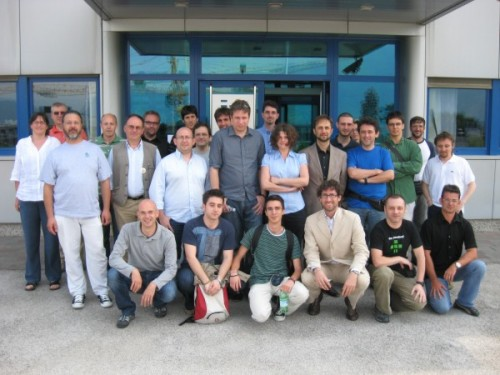
\includegraphics[width=0.55\columnwidth]{foto_gruppo_osmit.JPG}
 \caption{\textit{La foto di gruppo di OSMit 2009}}
\end{wrapfloat}
I \textbf{mapping party sono eventi legati a \osm}, un certo numero di OSMapper, sono così chiamati chi partecipa a \osm, sceglie una zona, solitamente poco mappata oppure da completare, incomincia a pubblicizzare l'evento all'interno della comunità e all'esterno contattando enti pubblici, associazioni e media per diffondere la manifestazione, il contatto esterno alla comunità è molto importante per cercare di coinvolgere nuove persone all'interno del progetto.

Solitamente i mapping party si tengono nel corso del weekend per cercare di far affluire più persone possibili, ricordo tra gli altri Mapping Party di Arezzo, il primo ufficiale in Italia, quello di Pompei, con scopi archeologici mappando all'interno dei resti romani della nota località napoletana, M(')appare Portofino, per la sentieristica del Parco naturale regionale di Portofino, Dolomiti Mapping Party, due giorni tra il gruppo del Brenta.
Inoltre \textbf{si possono realizzare anche eventi di durata minore, i micro mapping party} (Roma, Vicenza, Trentino, Milano). In Italia abbiamo anche sperimentato, con ottimi risultati, un mapping party dilatato nei mesi M(')appare Milano, con il supporto del trasmissione radiofonica Mentelocale di Radio Popolare di Milano e dell'associazione di volontariato GFOSS.it, sono stati organizzati per tre mesi micro mapping party con cadenza bisettimanale, questo ha permesso di andare a riempire molte zone del capoluogo lombardo e di diffondere il progetto.
\section{Informazioni utili}
\textbf{\url{http://wiki.openstreetmap.org/wiki/WikiProject_Italy} è il portale principale della comunità italiana}, per vedere il lavoro a livello nazionale e contattare gli altri utenti della penisola. È molto utile contribuire sul wiki attraverso \textbf{traduzioni} di pagine già esistenti in altre lingue, che servono sempre sia ai nuovi arrivati che a quelli che non conoscono al meglio la lingua inglese (la più usata sul wiki insieme al tedesco), sia alla \textbf{creazione e al mantenimento delle pagine} in italiano oltre a quelle della vostra regione, provincia o comune.

Esiste anche un sito in italiano che in questo momento è in fase di sviluppo \url{http://www.openstreetmap.it}; attualmente l'unica parte attiva è il blog \url{blog.openstreetmap.it}.

Tieni costantemente sotto controllo anche il portale wiki internazionale di \osm \url{http://wiki.openstreetmap.org/wiki/Main_Page} che contiene sempre ottimi spunti.  La comunità più attiva è quella tedesca con una marea di volontari (solo a Monaco di Baviera più di 200 mappatori) anche Gran Bretagna, Olanda e Svizzera hanno un'ottima copertura. In Italia il progetto è iniziato nel 2007 ed ora incomincia ad essere utilizzabile in special modo a livello locale e non globale poichè vi sono zone molto ben mappate e altre ancora vuote.

Se hai dubbi o domande consulta le risposte alle domande frequenti \url{http://wiki.openstreetmap.org/index.php/It:FAQ}, altri potrebbero aver avuto il tuo stesso problema e potresti trovare la soluzione.
\section{Contatti}
\textbf{Il principale riferimento nazionale è la mailing list italiana:\newline \url{http://lists.openstreetmap.org/listinfo/talk-it}}

Ci puoi trovare anche nella chat (canale irc) di GFOSS.it, la principale associazione che supporta OSM in italia. \#gfoss @ irc.eu.freenode.net 
È possibile accedervi via web grazie al servizio \url{webchat.freenode.net}  Canale \#gfoss

Esistono inoltre molti strumenti internazionali per svariate notizie su \osm \url{http://wiki.openstreetmap.org/wiki/Mailing_list}

\section{Software}
Di seguito verranno segnalati software, per diversi scopi, che hanno la possibilità di interfacciarsi con \osm.

\texttt{JOSM}: l'editor per \osm più utilizzato, scritto in java ha molti tools utilissimi oltre a svariati plugin

\texttt{Potlach}: editor online dal sito principale di \osm, molto comodo per la possibilità di avere le fotoaeree di Yahoo come sfondo

\texttt{Merkator}: altro editor per \osm

\texttt{Osmosis}: programma per gestire i dati di \osm

\texttt{QGIS}: software GIS per l'analisi e la visualizzazione di dati geografici, si interfaccia con \osm attraverso un plugin installabile dal manager del plugin in python

\texttt{PostgreSQL/PostGIS}: Database relazionale che con la sua estensione spaziale PostGIS può contenere i dati di \osm caricati utilizzando il software osm2pgsql

\texttt{Mapnik}: software per la rappresentazione di dati geografici, può creare singole immagini o tile per la pubblicazione sul web

\texttt{Osmarender}: simile al precedente

\texttt{Kosmos}: simile al precedente

\texttt{Qlandkarte}: software utilizzato soprattutto per la visualizzazione e la gestione di dati scaricati dal \gps, permette la visualizzazione come sfondo delle mappe di OSM

\texttt{MkGmap}: trasforma i dati in formato .osm in formato .img per Garmin

\texttt{Groudtruth}: simile al precedente

\texttt{Navit}: software per il routing con i dati di \osm

\texttt{Marble}: visualizzatore di dati geografici su modello Google Heart

\texttt{OSM3D}: visualizzatore 3D per i dati \osm

\section{Link}
\url{http://www.openstreetmap.org}: è il portale ufficiale di OSM. Da qui potrai consultare le mappe dimostrative “ufficiali” cliccando sul + in alto a destra sulla mappa:
Mapnik e Osmarender sono mappe generiche che mostrano molte caratteristiche mappate,
Cyclemap è invece una mappa tematica pensata per i ciclisti. Evidenzia le piste ciclabili nazionali, regionali e locali (ove mappate logicamente), le fontanelle di acqua potabile, i negozi di bici, le curve di livello e una colorazione pensata per mettere in risalto i rilievi.

\url{http://www.opencyclemap.org}: è il sito ufficiale della mappa sopra descritta.

\url{http://www.openpistemap.org}: è una mappa tematica pensata per gli amanti degli sport invernali, vengono renderizzati gli impianti di risalita, le piste a seconda della scala di difficoltà e le isolinee. 

%\url{http://www.openferrymap.org}: %CONTROLLARE SE È GIUSTO 
%mappa tematica che visualizza le ferrovie e gli elementi legati a questa tipologia di trasporto pubblico

\url{http://www.openseamap.org}: mappa tematica che visualizza gli elementi utili alla navigazione

\url{http://www.yournavigation.org}: si tratta di un navigatore che permette di trovare il percorso migliore che unisce due punti. E' possibile scegliere il più breve, il più veloce o l'utilizzo a piedi o in bicicletta. I percorsi trovati per la bici daranno priorità alle piste ciclabili.

\url{http://www.openrouteservice.org}: il servizio principale proposto è un navigatore simile a quello sopra descritto. In Germania, basandosi sul servizio strade è capace di calcolare in tempo reale il percorso migliore in base al traffico od eventuali incidenti. Il sito fornisce inoltre servizi più specifici come ad esempio il tempo di accessibilità: dato un punto sulla mappa verrà evidenziata l'area raggiungibile entro un determinato tempo dal punto considerato.

\url{http://www.openstreetbrowser.org}: è un che permette di visualizzare innumerevoli informazioni inserite in \osm, altrimenti nascoste o visibili soltanto mediante un rendering ad hoc. Ne sono un esempio l'evidenziamento dinamico dei percorsi dei mezzi pubblici con le relative fermate, ma anche strutture turistiche, storiche, sportive. E' nato da poco, ancora in versione sperimentale. Può avere qualche malfunzionamento.

\url{http://www.itoworld.com}: è una azienda che fornisce un utile servizio per verificare l'attività di mappatura in una determinata zona: scoprire  e contattare gli utenti che ci lavorano, vedere le modifiche nel tempo. Necessita di registrazione gratuita.

\url{http://www.cloudmade.com}: fornisce svariati servizi come ad esempio, previa registrazione, la possibilità di creare in modo semplice mappe con rendering personalizzato.

\url{http://www.geofabrik.de}: fornisce svariati servizi come la possibilità di scaricare i dati osm relativi ad una determinata nazione e un tool per confrontare le mappe \osm con le mappe di google. Si scoprirà come in molti casi la precisione e il dettaglio di osm siano superiori a googlemaps. Le mappe di google devono essere utilizzate solo come interessante confronto e non per essere copiate.

\url{http://walking-papers.org}: permette di stampare una mappa da utilizzare durante le ``mappature'' per segnare nuovi elementi, inoltre una volta scannerizzato il foglio con le modifiche si può inserire sul portale
\newpage
\begin{center}\begin{small}\textbf{
Questo documento è rilasciato con licenza 
Creative Commons Attribution No Commercial Share Alike
\url{http://creativecommons.org/licenses/by-nc-sa/2.5/it/}}\end{small}\end{center}
\begin{center}
 
\includegraphics{ccbysa.png}
\end{center}
\end{document}
